\Chapter{Resultaten\label{hfdst-resultaten}}

In dit hoofdstuk zal het ASIC ontwerp van de schakeling die in \refhfdst{hfdst-implementatie} beschreven werd van naderbij bestudeerd worden. Daarbij zal gekeken worden naar de oppervlakte van de schakeling, het verbruik en de maximum bereikbare kloksnelheid $f_{\text{max}}$. Er zal onderzocht worden wat het effect van de verschillende voorgestelde optimalisaties is op al deze parameters. Ten slotte zal het ontwerp vergeleken worden met reeds bestaande implementaties.

Het ontwerp werd geprogrammeerd in GEZEL \cite{gezel}. Simulaties en compilatie naar VHDL werden uitgevoerd met GEZEL 2.0. De optimalisaties werden doorgevoerd in de VHDL code, aangezien GEZEL dit niet toelaat. Alle ontwerpen werden gesynthetiseerd met behulp van Synopsys Design Vision. De gebruikte bibliotheek was de \emph{$0.13 \mu m$ low leakage} bibliotheek van Faraday Technology \cite{cell-databook}. Het werd de software verboden flip-flops met test ingangen te gebruiken. De maximale oppervlakte werd ingesteld op nul, wat als netto effect een resultaat met minimum oppervlakte gaf. Verder werd voor het kloksignaal een frequentie van 10kHz gedefini\"eerd.

De grootte van alle resultaten wordt uitgedrukt in gates. Dit laat toe te vergelijken met andere resultaten die in de literatuur terug te vinden zijn.

Voor de resultaten in verband met energieverbruik worden steeds twee waarden gegeven. De eerste waarde, dynamisch verbruik, geeft weer hoeveel vermogen verbruikt wordt door veranderende CMOS in- en uitgangen. De tweede waarde, leakage verbruik, is verbruik dat voorkomt zelfs indien een transistor niet geleidt. De impact hiervan hangt onder meer af van de gebruikte bibliotheek.

Deze beide waarden moeten met een stevige korrel zout genomen worden. Het is voor het synthese programma zeer moeilijk hier een nauwkeurige schatting voor te geven. Zolang twee schakelingen echter met dezelfde software, bibliotheek en parameters werden gesynthetiseerd, zijn relatieve vergelijkingen mogelijk. Stel bijvoorbeeld dat het verbruik van ontwerp A geschat wordt op $200 nW$ en dit van ontwerp B op $100 nW$. Indien er dan voldaan is aan de voorgenoemde voorwaarden, zal het effectief verbruik van B ongeveer de helft zijn van A. Het is dus in het algemeen niet aangeraden vergelijkingen omtrent verbruik te maken met andere bestaande ontwerpen aan de hand van de waarden gegeven in dit hoofdstuk.

% TODO: Blijft leakage constant bij hogere kloksnelheid?

Indien gewenst kan het verbruik voor hogere kloksnelheiden geschat worden. Gegeven de standaard frequentie $f = 10$kHz, de formule voor het dynamisch verbruik van een CMOS schakeling:
\[P_d = V^2 \cdot C \cdot f\]
en het leakage verbruik $P_l$, kan men dus het totale verbruik omrekenen naar dat van een willekeurige kloksnelheid via
\[P' = \frac{P_d \cdot f'}{10 000} + P_l.\]

\section{Basisimplementatie \& register optimalisaties\label{section-resultaten-basisimplementatie}}

Het synthetiseren van de meest eenvoudige implementatie, zonder enige optimalisaties aan de registers en met slechts \'e\'en MALU in de $\mathbb{F}_{2^m}$ kern, geeft de resultaten in \reftbl{tabel-resultaten-basis}.

\begin{table}[h]
	\caption{Syntheseresultaten voor de basis implementatie}
	\label{tabel-resultaten-basis}

	\centering
	\begin{tabular}{|l|l|l|l|}
		\hline
		\multirow{2}{*}{Opp. (gates)}	& \multicolumn{2}{c|}{Verbruik @ 10kHz ($nW$)}	& \multirow{2}{*}{$f_{\text{max}}$ (MHz)}\\
		\cline{2-3}
		& Dynamisch	& Leakage	& \\
		\hline
		$31\:943$	& 515	& 134	& 53.22\\
		\hline		
	\end{tabular}
\end{table}

Deze resultaten zullen nu vergeleken worden met de verschillende register optimalisaties. Bij de implementaties van clock gating wordt steeds ook de reset ingangen van zoveel mogelijk registers verwijderd. De synthese resultaten voor de vier verschillende optimalisaties worden gegeven in \reftbl{tabel-resultaten-optimalisaties}. Zoals verwacht verbruiken al deze resultaten minder dan de niet-geoptimaliseerde versie. De versies met clock gating (CG $n$) implementeren de schakelingen in de volgorde waarin ze voorkomen in \refsect{subsectie-implementatie-optimalisatie-clock-gating}. Voor elke parameter wordt aangegeven hoeveel deze beter is dan in de niet-geoptimaliseerde versie. Ter verduidelijking zijn de oppervlakte en het totale verbruik van deze resultaten ook nog eens uitgezet in \reffig{figuur-resultaten-m1}.

\begin{table}[h]
	\caption{Syntheseresultaten voor de register optimalisaties}
	\label{tabel-resultaten-optimalisaties}

	\centering
	\begin{tabular}{|l|lr|lr|lr|lr|}
		\hline
		& \multicolumn{2}{l|}{\multirow{2}{*}{Opp. (gates)}}	& \multicolumn{4}{c|}{Verbruik @ 10kHz ($nW$)}	& \multicolumn{2}{l|}{\multirow{2}{*}{$f_{\text{max}}$ (MHz)}}\\
		\cline{4-7}
		&	& & \multicolumn{2}{l|}{Dynamisch}	& \multicolumn{2}{l|}{Leakage}	& &\\
		\hline \hline
		Basis			& $31\:943$	& & 515	& 	& 134 & 	& 53.22 & \\
		\hline
		Geen reset	& $33\:221$	& 1\%	& 473	& 5\%	& 134 & 0\%	& 54.08	& 2\%\\
		CG 1			& $30\:481$	& 1\%	& 104	& 5\%	& 117	& 5\%	& 47.73	& 5\%\\
		CG 2			& $30\:481$	& 1\%	& 104	& 5\%	& 117	& 5\%	& 47.73	& 5\%\\
		CG 3			& $30\:481$	& 1\%	& 104	& 5\%	& 117	& 5\%	& 47.73	& 5\%\\
		\hline		
	\end{tabular}
\end{table}

\begin{figure}[h]
	\centering
		\fbox{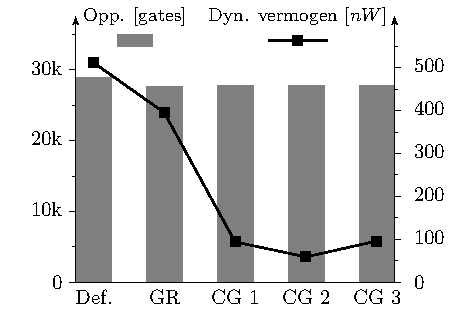
\includegraphics[scale=1]{results-m1}}
		\caption{Syntheseresultaten voor de basis implementatie met en zonder register optimalisaties\label{figuur-resultaten-m1}}
\end{figure}

\section{Meerdere MALU's\label{sectie-resulaten-malus}}

Mits de toevoeging van extra MALU's is het mogelijk de totale rekeningtijd drastisch te verlagen (zie \refsect{subsectie-implementatie-gf2m-versnelling}). Hoewel het gebruik van meerdere MALU's de uiteindelijke schakeling vergroot en dat dus enigszins in gaat tegen de originele doelstelling, wordt hier toch onderzocht in welke mate de interessante parameters hierdoor juist worden be\"invloed. Er kan dan een afweging gemaakt worden tussen het gebruik van een schakeling met \'e\'en MALU op hogere kloksnelheid versus \'e\'en met meerdere MALU's aan een lagere kloksnelheid. De eerste schakeling zal kleiner zijn, maar waarschijnlijk wel meer verbruiken dan de tweede.

De totale berekeningstijd $t = \frac{c}{f}$ kan bepaald worden in functie van het aantal benodigde klokcycli $c$ en het aantal MALU's $d$:
\[c = 27058 + 2993 \cdot \left\lceil \frac{163}{d} \right\rceil,\]
waarbij 2993 het aantal vermenigvuldigingen is dat dient uitgevoerd te worden en de tweede term in de vermenigvuldiging het aantal klokcycli is dat een vermenigvuldiging kost. In \reftbl{tabel-resultaten-multi-cycles} wordt voor enkele waarden getoond hoeveel klokcycli nodig zijn om een berekening te voltooien. In \reffig{figuur-resultaten-multi-cycles} wordt hetzelfde weergegeven, maar dan voor elke $d$ van 1 t.e.m.\ 163. Het is duidelijk dat de tijdsbesparing waar extra MALU's voor zorgen vrij snel teniet wordt gedaan door het aantal cycli dat niet door $d$ be\"invloed wordt.

\begin{table}[h]
	\caption{Aantal klokcycli $c$ nodig voor \'e\'en pairing i.f.v.\ aantal MALU's $d$}
	\label{tabel-resultaten-multi-cycles}

	\centering
	\begin{tabular}{|l||l|l|l|l|l|l|l|l|}
		\hline
		$d$	& 1	& 2	& 3	& 4	& 6	& 8	& 16	& 32\\
		\hline
		$c$	& $514\:917$	& $272\:484$	& $191\:673$	& $149\:771$	& $110\:862$	& $89\:911$	& $59\:981$	& $45\:016$\\
		\hline		
	\end{tabular}
\end{table}

\begin{figure}[h]
	\centering
		\fbox{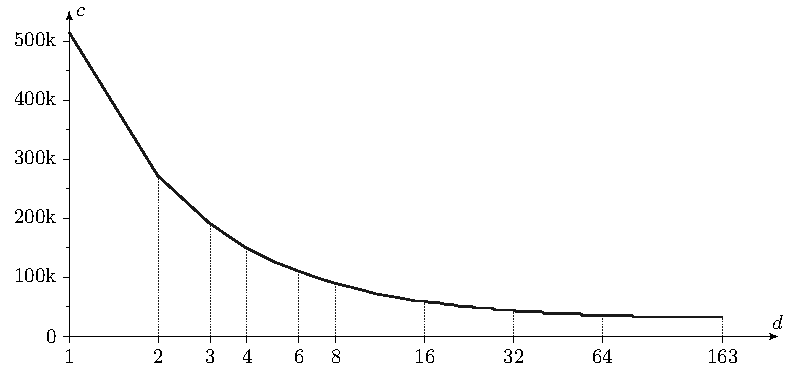
\includegraphics[width=\textwidth]{results-multi-cycles}}
		\caption{Aantal klokcycli $c$ nodig voor \'e\'en pairing i.f.v.\ aantal MALU's $d$\label{figuur-resultaten-multi-cycles}}
\end{figure}

Op de implementaties met meerdere MALU's werden ook steeds de derde clock gating techniek (en het verwijderen van reset ingangen) toegepast, aangezien deze de grootste energiebesparing teweeg brengt. Implementaties met een aantal MALU's gaande van twee t.e.m.\ twee\"endertig werden gesynthetiseerd. Een nog hoger aantal MALU's zou immers compleet ingaan tegen de originele doelstelling. De resultaten van de synthese zijn te zien in \reftbl{tabel-resultaten-md} en \reffig{figuur-resultaten-md}. Indien men nog meer snelheidswinst wenst te boeken, zou het beter zijn het gehele ontwerp anders te ontwikkelen (bv.\ door RAM te gebruiken i.p.v.\ individuele registers).

\begin{table}[h]
	\caption{Syntheseresultaten voor meerdere MALU's}
	\label{tabel-resultaten-md}

	\centering
	\begin{tabular}{|l||l@{$\:$}r|lr|lr|l@{$\:$}r|l|}
		\hline
		\multirow{2}{*}{$d$} & \multicolumn{2}{l|}{\multirow{2}{*}{Opp. (gates)}}	& \multicolumn{4}{c|}{Verbruik @ 10kHz ($nW$)}	& \multicolumn{2}{l|}{\multirow{2}{*}{$f_{\text{max}}$ (MHz)}} & \multirow{2}{1cm}{Tijds-\\winst}\\
		\cline{4-7}
		&	& & \multicolumn{2}{l|}{Dynamisch}	& \multicolumn{2}{l|}{Leakage}	& & &\\
		\hline \hline
		1			& $30\:481$	& 100\%	& 104	& 100\%	& 117	& 5\%	& 47.73	& 100\%	& 0\%\\
		\hline
		2			& $30\:481$	& 1\%	& 104	& 5\%	& 117	& 5\%	& 47.73	& 5\%	& 47.1\%\\
		3			& $30\:481$	& 1\%	& 104	& 5\%	& 117	& 5\%	& 47.73	& 5\%	& 62.8\%\\
		4			& $30\:481$	& 1\%	& 104	& 5\%	& 117	& 5\%	& 47.73	& 5\%	& 70.9\%\\
		6			& $30\:481$	& 1\%	& 104	& 5\%	& 117	& 5\%	& 47.73	& 5\%	& 78.5\%\\
		8			& $30\:481$	& 1\%	& 104	& 5\%	& 117	& 5\%	& 47.73	& 5\%	& 82.5\%\\
		16			& $30\:481$	& 1\%	& 104	& 5\%	& 117	& 5\%	& 47.73	& 5\%	& 88.4\%\\
		32			& $30\:481$	& 1\%	& 104	& 5\%	& 117	& 5\%	& 47.73	& 5\%	& 91.3\%\\
		\hline		
	\end{tabular}
\end{table}

\begin{figure}[h]
	\centering
		\fbox{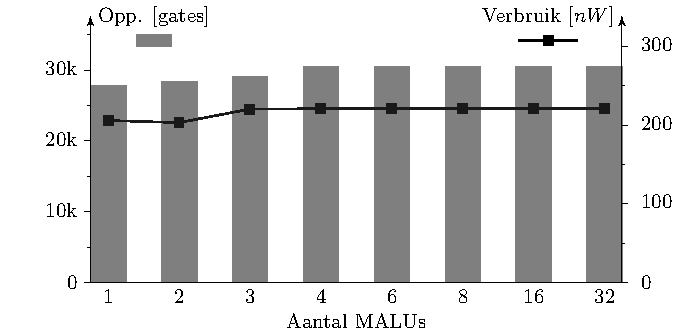
\includegraphics[scale=1]{results-md}}
		\caption{Syntheseresultaten voor implementaties met meerdere MALU's\label{figuur-resultaten-md}}
\end{figure}

\section{Hogere kloksnelheid vs.\ meerdere MALU's}

Aan de gegeven kloksnelheid van 10kHz doet een schakeling met \'e\'en MALU er 51.5 seconden over om \'e\'en pairing te berekenen. Dit zal  in de meeste gevallen onaanvaardbaar zijn. Daarom wordt hier onderzocht wat de effecten op de schakeling zijn indien de kloksnelheid wordt opgedreven en er eventueel meerdere MALU's gebruikt worden. Aangezien het doel nog steeds blijft de schakeling zo klein mogelijk te maken, zal voor een implementatie met meerdere MALU's enkel die met twee nader onderzocht worden.

Stel een maximale rekentijd $t_{\text{max}} = 50ms$. Voor een implementatie met \'e\'en MALU moet de klokfrequentie $f_1$ dan 1030 maal verhoogd worden. Wanneer men de schakeling met twee MALU's even snel wenst te maken als die met \'e\'en dan dient de kloksnelheid $f_2$ van die eerste vermenigvuldigd te worden met:
\[\begin{aligned}
\Delta f &= \frac{272484}{514917}\\
	&= 0.52918.
\end{aligned}\]
De kloksnelheden van de respectievelijke schakelingen zijn dan:
\[\begin{aligned}
f_1	&= 10.3\text{MHz}\\
f_2	&\approx 5.45\text{MHz}.
\end{aligned}\]

Ter vergelijking worden de resulterende parameters van beide implementaties gegeven in \reftbl{tabel-resultaten-m1-vs-m2}. Beiden werden volledig gehersynthetiseerd met aangepaste parameters voor de klok. De schattingen voor het vermogen zijn dus niet bekomen door de conversie formule aan het begin van dit hoofdstuk toe te passen. Welke van de twee opties de voorkeur zal genieten, zal afhangen van toepassing tot toepassing.

\begin{table}[h]
	\caption{Vergelijking van syntheseresultaten voor twee verschillende implementaties die er even lang over doen \'e\'en pairing te berekenen}
	\label{tabel-resultaten-m1-vs-m2}

	\centering
	\begin{tabular}{|l|l|l@{\;\;}l|}
		\hline
		& 1 MALU	& \multicolumn{2}{l|}{2 MALU's}\\
		\hline \hline
		Opp. (gates)	& $30\:481$	& $30\:481$	& 120\% \\ \hline
		$f$ (MHz)		& 10.3		& 5.45		& 52.9\% \\ \hline
		Verbruik ($nW$)& 				& 				& \\
		$\quad$ Dynamisch	& 104			& 134			& 118\% \\
		$\quad$ Leakage	& 114			& 164			& 144\% \\ \hline
		$f_{\text{max}}$ (MHz)	& 47.73	& 40.12	& 85\% \\
		\hline		
	\end{tabular}
\end{table}

\section{Vergelijking met bestaande implementaties}

Gezien de vrij recente ontwikkeling van pairings lag de focus tot nu toe steeds op het snel berekenen van de pairing. Enkele papers beschrijven een ontwerp voor gebruik in sensor netwerken. Helaas hebben deze allemaal als doelplatform een microprocessor. Er werd slechts \'e\'en paper gevonden waarin het uiteindelijke resultaat naar een ASIC gesynthetiseerd werd. Alle andere recent gepubliceerde implementaties werden ontwikkeld in software of voor FPGA's. Gezien de eerder vermelde focus op snelheid wordt in die gevallen nooit vermeld hoeveel de uiteindelijke schakelingen verbruiken.

Het is dus zo goed als onmogelijk een grondige vergelijking te maken tussen de verschillende bestaande implementaties, gezien hun volledig andere invalshoek. Toch zal zo goed als mogelijk getracht worden enigszins een overzicht te geven, zodat de in deze thesis voorgestelde schakeling beter geplaats kan worden tussen de reeds bestaande ontwerpen.

De ontwerpen specifiek gericht op sensor netwerken worden voorgesteld in \cite{tinypbc, tinytate, nanoecc}. In alle gevallen wordt de pairing berekend op een ATMega128L microchip. Deze implementaties zijn ontwikkeld voor gebruik op een MICA node, specifiek ontwikkeld voor gebruik in sensor netwerken. Een overzicht van de resultaten is gegeven in \reftbl{tabel-resultaten-sensor}. Rekening houdend met het stroomverbruik gegeven in \cite{nanoecc} wordt het verbruik tijdens een berekening geschat op ongeveer $23.60mW$. Uiteraard zijn de oppervlakte en het verbruik van een microchip implementatie niet te vergelijken met de in deze thesis voorgestelde ASIC schakeling, gezien de zeer verschillende filosofie achter het gebruik van beiden.

\begin{table}[h]
	\caption{Resultaten voor bestaande ontwerpen met focus op sensor netwerken}
	\label{tabel-resultaten-sensor}

	\centering
	\begin{tabular}{|l|l|p{1cm}|}
		\hline
		& Pairing	&	Reken-tijd ($s$)\\
		\hline \hline
		NanoECC \cite{nanoecc}		& $e(\mathbb{F}_{2^{163}})$	& 10.96\\
		NanoECC \cite{nanoecc}		& $e(\mathbb{F}_{q = 160})$	& 17.93\\
		TinyTate \cite{tinytate}	& $e(\mathbb{F}_{q = 256})$	& 30.21\\
		TinyPBC	\cite{tinypbc}		& $\eta_T(\mathbb{F}_{2^{271}})$	& 5.45\\
		\hline		
	\end{tabular}
\end{table}

Toch wordt in \reftbl{tabel-resultaten-andere} een overzicht gegeven van enkele van deze implementaties om een idee te geven over tot nu toe gepubliceerde resultaten.

zijn er in de literatuur niet heel veel implementaties terug te vinden. De weinige papers die over implementaties handelen zijn verder steeds gefocussed op snelheid. Verder was er ten tijde van schrijven geen ander ASIC ontwerp bekend. Daar alle andere hardware implementaties of voor microchip of voor FPGA ontwikkeld zijn, is het zeer moeilijk onderbouwde conclussies te trekken. Toch worden in enkele andere ontwerpen voorgesteld. Voor het stroomverbruik werd uitgegaan van het gemiddeld verbruik opgegeven door de fabrikant.

\begin{table}[h]
	\caption{Resultaten uit de literatuur voor verschillende implementaties van pairings}
	\label{tabel-resultaten-andere}

	\centering
	\begin{tabular}{|l||l|l|l|l|l|l|}
		\hline
		&	Platform	& Curve	& Verbruik ($W$)	& $f$ (MHz)	& Rekentijd ($\mu s$)\\
		\hline
	\end{tabular}
\end{table}
